\documentclass{article}
\usepackage{graphicx}
\usepackage{pgfplots}

\usepackage{tikz}
\usepackage{circuitikz}



\begin{document}

\begin{titlepage}
    \begin{center}
        \vspace*{1cm}
 
        \Huge
        \textbf{project Title}
 
        \vspace{0.5cm}
        \LARGE
        Databae Managment System
 
        \vspace{1.5cm}
 
        \textbf{Author:Zarin Jahan Shazi}
        
        \vfill
       
        \line(1,0){300}\\
        \huge{\bfseries My First Report}
 		\line(1,0){200}
 
        \vspace{0.8cm}
 
        {ID:18ictcse049}
 
        \Large
        Dept Of CSE\\
        Bangubangu Sheikh Mujibur Rahman Science and Technology University(SHIICT)\\
        Bangladesh\\
        26th january 2020
 
    \end{center}
\end{titlepage}
\newpage
% front matter stuff
\pagenumbering{roman}
\section*{summary}
\addcontentsline{toc}{section}{\numberline{}summary}
This PDF describes writing report using latex.
\cleardoublepage
\section*{Acknowledgement}
\addcontentsline{toc}{section}{\numberline{}Acknowledgements}
Thank you
\cleardoublepage
% table of contents
\tableofcontents
\thispagestyle{empty}
\cleardoublepage
%main body stuff
\pagenumbering{arabic}
\setcounter{page}{1}

\section{Introduction}
\line(1,0){400}\\
 A database management system (DBMS) is system software for creating and managing databases. A DBMS makes it possible for end users to create, read, update and delete data in a database. The most prevalent type of data management platform, the DBMS essentially serves as an interface between databases and end users or application programs, ensuring that data is consistently organized and remains easily accessible.
 \newpage
\section{History}
\line(1,0){400}\\
The sizes, capabilities, and performance of databases and their respective DBMSs have grown in orders of magnitude. These performance increases were enabled by the technology progress in the areas of processors, computer memory, computer storage, and computer networks. The development of database technology can be divided into three eras based on data model or structure: navigational,[8] SQL/relational, and post-relational.

The two main early navigational data models were the hierarchical model and the CODASYL model (network model)

The relational model, first proposed in 1970 by Edgar F. Codd, departed from this tradition by insisting that applications should search for data by content, rather than by following links. The relational model employs sets of ledger-style tables, each used for a different type of entity. Only in the mid-1980s did computing hardware become powerful enough to allow the wide deployment of relational systems (DBMSs plus applications). By the early 1990s, however, relational systems dominated in all large-scale data processing applications, and as of 2018 they remain dominant: IBM DB2, Oracle, MySQL, and Microsoft SQL Server are the most searched DBMS.[9] The dominant database language, standardised SQL for the relational model, has influenced database languages for other data models.[citation needed]

Object databases were developed in the 1980s to overcome the inconvenience of object-relational impedance mismatch, which led to the coining of the term "post-relational" and also the development of hybrid object-relational databases.

The next generation of post-relational databases in the late 2000s became known as NoSQL databases, introducing fast key-value stores and document-oriented databases. A competing "next generation" known as NewSQL databases attempted new implementations that retained the relational/SQL model while aiming to match the high performance of NoSQL compared to commercially available relational DBMSs.
 

\newpage
\section{Functions of a DBMS}
\line(1,0){400}\\
The DBMS manages three important things: the data, the database engine that allows data to be accessed, locked and modified, and the database schema, which defines the database's logical structure. These three foundational elements help provide concurrency, security, data integrity and uniform data administration procedures. Typical database administration tasks supported by the DBMS include change management, performance monitoring and tuning, security, and backup and recovery. Many database management systems are also responsible for automated rollbacks and restarts as well as the logging and auditing of activity in databases.
The DBMS is perhaps most useful for providing a centralized view of data that can be accessed by multiple users, from multiple locations, in a controlled manner. A DBMS can limit what data the end user sees, as well as how that end user can view the data, providing many views of a single database schema. End users and software programs are free from having to understand where the data is physically located or on what type of storage media it resides because the DBMS handles all requests.

The DBMS can offer both logical and physical data independence.This means it can protect users and applications from needing to know where data is stored or having to be concerned about changes to the physical structure of data. As long as programs use the application programming interface (API) for the database that is provided by the DBMS, developers won't have to modify programs just because changes have been made to the database.

In a relational database management system (RDBMS), the most widely used type of DBMS, this API is SQL, a standard programming language for defining, protecting and accessing data in an RDBMS.

\begin{figure}[h]
\centering
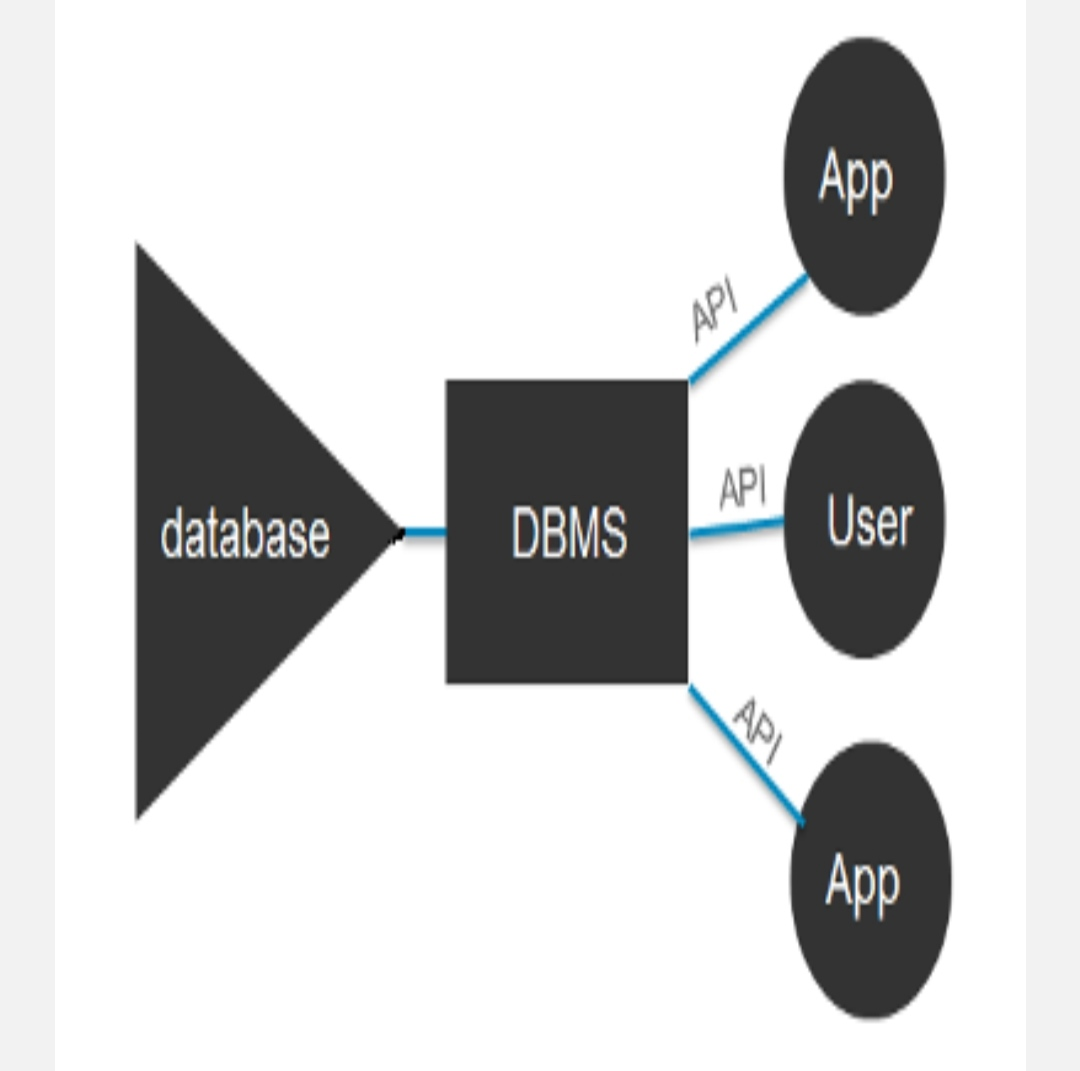
\includegraphics[width=\linewidth5]{1.jpg}

\caption{Functions}
\end{figure}






\newpage
\section{Popular types of DBMS technologies}
\line(1,0){300}\\
Popular database models and management systems include:

Relational database management system (RDBMS) -- adaptable to most use cases, but RDBMS Tier-1 products can be quite expensive.
NoSQL DBMS -- well-suited for loosely defined data structures that may evolve over time.
In-memory database management system (IMDBMS) -- provides faster response times and better performance.
Columnar database management system (CDBMS) -- well-suited for data warehouses that have a large number of similar data items.
\begin{figure}[h]
\centering
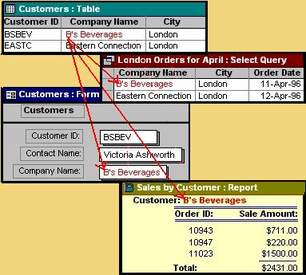
\includegraphics[width=\linewidth5]{2.jpg}

\caption{database}
\end{figure}
Cloud-based database management system -- the cloud service provider is responsible for providing and maintaining the DBMS.




\newpage
\section{Advantages of using a DBMS}
\line(1,0){300}\\
Using a DBMS to store and manage data comes with advantages, but also processing overhead. One of the biggest advantages of using a DBMS is that it lets end users and application programmers access and use the same data while managing data integrity. Data is better protected and maintained when it can be shared using a DBMS instead of creating new iterations of the same data stored in new files for every new application. The DBMS provides a central store of data that can be accessed by multiple users in a controlled manner.

Central storage and management of data within the DBMS provides:

Data abstraction and independence.
Data security.
A locking mechanism for concurrent access.
An efficient handler to balance the needs of multiple applications using the same data.
The ability to swiftly recover from crashes and errors, including restartability and recoverability.
Robust data integrity capabilities.
Logging and auditing of activity.
Simple access using a standard API.
Uniform administration procedures for data.
Another advantage of a DBMS is that it can be used to impose a logical, structured organization on the data. A DBMS delivers economy of scale for processing large amounts of data because it is optimized for such operations.
\begin{figure}[h]
\centering
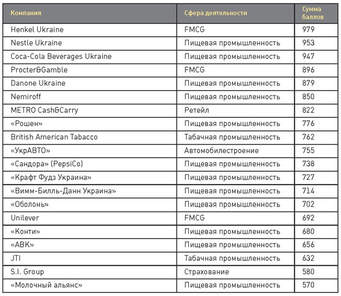
\includegraphics[width=\linewidth5]{3.jpg}

\caption{database}
\end{figure}

A DBMS can also provide many views of a single database schema. A view defines what data the user sees and how that user sees the data. The DBMS provides a level of abstraction between the conceptual schema that defines the logical structure of the database and the physical schema that describes the files, indexes and other physical mechanisms used by the database. When a DBMS is used, systems can be modified much more easily when business requirements change. New categories of data can be added to the database without disrupting the existing system and applications can be insulated from how data is structured and stored.

However, a DBMS must perform additional work to provide these advantages, thereby bringing with it the overhead. A DBMS will use more memory and CPU than a simple file storage system, and different types of DBMSes will require different types and levels of system resources.

\newpage
\section{Changes in how DBMSes are built, sold and serviced}
\line(1,0){400}\\
    By 2019, the most significant trends in the DBMS sector were how databases were constructed and how they were used. Open source DBMS technologies were rapidly gaining traction. In fact, Gartner projected that open source databases would account for 10% of total spending on database software by 2019 due to increased enterprise adoption. Most mainstream IT organizations use open source software in some of their mission-critical operations.


This trend complements two others: the acquisition of open-source database vendors by bigger rivals and the expansion of the cloud-based database service market. For example, in 2019, MongoDB, maker of the Atlas cloud platform based on its namesake NoSQL DBMS, acquired mobile app database maker Realm to boost its abilities in the mobile computing landscape. Also, Microsoft acquired Citus Data, whose open source software allows PostgreSQL to be used as a distributed database in a public cloud setting.

In 2019, Gartner also said that cloud databases are now driving most of the growth in the DBMS market, describing the cloud as "the default platform for managing data." In connection with the increasing shift toward the cloud, numerous DBMS vendors have introduced managed cloud database services that offer to free IT and data management teams from having to deploy, configure and administer database systems themselves.
\newpage
 \section{Add Table}
 \line(1,0){200}\\




    \begin{tabular}{|c|c|c|c|}
    \hline
    Nafisa Zaman &Mouli Afrin &Israt Jahan &Zannatul Mim\\\hline
    id:01 &id:01 &id:03 &id:04\\\hline
    cgpa:2.55 &cgpa:3.55 &cgpa:4.00 &cgpa:3.78\\\hline
    \end{tabular}\\
  	[8 cm]
\subsection{Add Graph}
\begin{tikzpicture}[>=stealth]
    \begin{axis}[
        xmin=-4,xmax=4,
        ymin=-2,ymax=2,
        axis x line=middle,
        axis y line=middle,
        axis line style=<->,
        xlabel={$x$},
        ylabel={$y$},
        ]
        \addplot[no marks,blue,<->] expression[domain=-pi:pi,samples=100]{sin(deg(2*x))+1/2} 
                    node[pos=0.65,anchor=south west]{$y=\sin(2x)+\frac{1}{2}$}; 
    \end{axis}
\end{tikzpicture}
\newpage
\subsubsection{Add Circuit}
 

  \begin{circuitikz}
      \draw (0,0)
      to[V,v=$U_q$] (0,2) % The voltage source
      to[short] (2,2)
      to[R=$R_1$] (2,0) % The resistor
      to[short] (0,0);
      \draw (2,2)
      to[short] (4,2)
      to[L=$L_1$] (4,0)
      to[short] (2,0);
      \draw (4,2)
      to[short] (6,2)
      to[C=$C_1$] (6,0)
      to[short] (4,0);
   \end{circuitikz}
   \section{Mathemetical Equation}
   % change this line to \documentclass{article} or whatever you want.


\noindent
The square root of 100 is $\sqrt{100}=10$. 
\\
But the cubic root of 64 is $\sqrt[3]{64}=4$.










\end{document}



